\documentclass[../main.tex]{subfiles}
\begin{document}
	\section{Евклидовы и унитарные пространства}
	\subsection{Скалярное, псевдоскалярное произведение в Евкл. и унитарном про-вах. Норма в Евклидовом и унитарном пространствах.}
	\begin{defin}
		$V$ -- линейное пространство над $\R$ (вещ. пр-во)\n
		$(\cdot, \cdot): V\times V \rightarrow \R$\n
		Скалярное произведение, если удовлетворяет 4м \textbf{аксиомам:}\n
		$\begin{matrix}
		\forall x, y \in V\\
		\forall \lambda \in \R
		\end{matrix}: $
		\begin{mylist}
			\item 
			$(x, y) = (y, x)$ (симметр.)
			\item 
			$(x+y, z) = (x, z) + (y, z)$ (Аддитивность по первому аргументу)
			\item $(\lambda x, y) = \lambda (x, y)$ (Однородность по первому аргументу)
			\item $\forall x \neq 0 \; (x, x) > 0 $ (Положительная определенность)
		\end{mylist}
		Из этих свойств можно понять, что скал. произведение -- билинейная функция.\\
		Из 3 $\Rightarrow \forall x \in V \; \; (x, \0) = (\0, x) = 0$\\
		Из 4 $\Rightarrow \forall x \in V \; \; (x, x) \geq 0$, причем $= 0 \Leftrightarrow x = \0$
	\end{defin}
	\begin{defin}
		$V$ конечномерное, линейное пространство над $\R$\\
		$(V, (\cdot, \cdot))$ -- \textbf{Евклидово пространство}
	\end{defin}
	\begin{remark}
		$V$ бесконечномерное $(X, (\cdot, \cdot))$ \textbf{предгильбертово}\\
		Если полное метрическое пространство, то оно называется \textbf{гильбертовым}\\
		(Полное -- любая фундаментальная последовательность сходится, из матанализа)
	\end{remark}
	\begin{defin}
		$V$ -- линейное пространство над полем $\mathbb C$ (комплексн. линейное пространство)\\
		$(\cdot, \cdot) : V \times V \rightarrow \mathbb{C}$\\
		\textbf{Псевдоскалярное произведение: }\\
		$\begin{matrix}
			\forall x, y, z \in V \\
			\forall \lambda \in \mathbb C
		\end{matrix}$:
		\begin{mylist}
			\item $(x, y) = \vec{(y, x)}$
			\item $(x + y, z) = (x, z) + (y, z)$ (Аддитивность)
			\item $(\lambda x, z) = \lambda ( x, z) $ (Однородность по 1му аргументу)
			Из 2 и 3 $\Rightarrow$ линейность по 1 аргументу
			\item $\forall x \neq 0 \; \; (x, x) > 0$ (Положительная определенность)
		\end{mylist}
		1, 2, 3    $\; \; \; (x, y+z) = \vec{(y + z, x)} = \vec{(y, x)} + \vec{(z, x)} = (x, y) + (x, z)\\
		\; \; \; \; (x, \lambda y) = \vec{(\lambda y, x)} = \vec \lambda \vec{(y, x)}$ Псевдооднородность по 2 арг.\n
		$\underset{\leftrightarrow}{(x, x)} = \vec{(x, x)} \leftrightarrow (x, x) \in \R\n
		\forall x \in V \; \; (x, x) \geq 0$, причем $=0 \Leftrightarrow x = 0$
	\end{defin}
	\begin{defin}
		Конечномерное $V$ над полем $\mathbb C$ \\
		$(X, (\cdot, \cdot))$ называется \textbf{унитарными} (псевдоевклидовым, эрмитовым)
	\end{defin}
	\begin{defin}
		$(V, (\cdot, \cdot))$ Евклидово (унит.) пространство\n
		$\underset{\text{\textbf{норма}}}{||\cdot||}: V \rightarrow \R_+ \; \; \forall x \in V \; ||x|| = \sqrt{(x, x)} \; \;$ \textbf{Евклидова норма}\n
		\textbf{Аксиомы нормы:}
		\begin{mylist}
			\item 
			$||x|| = 0 \Rightarrow x = \0$ (невырожденность)
			\item $||\lambda x|| = |\lambda| ||x||$ (однородность)
			\item $||x+y|| \leq ||x|| + ||y||$ (неравенство треугольника)
		\end{mylist}
	\end{defin}
		$||x|| = \sqrt{(x, x)}$\\
		Ввели такую норму, удостоверимся, что все аксиомы выполнены:
		\begin{mylist}
			\item Очевидно из 4
			\item $\sqrt{(\lambda x, \lambda x)} = \sqrt{\underset{|\lambda|^2}{\lambda \vec \lambda}(x, x)} = |\lambda| \sqrt{(x, x)} = |\lambda| ||x||$
			\item ?\\
			Давайте докажем неравенство Коши-Буняковского-Шварца\\
			$\forall x, y \in (V, (\cdot, \cdot)) \; \; |(x, y)| \leq ||x||\cdot||y||$\\
			2) Причем $= \Leftrightarrow x$ и $y$  линейно зависимы
			\begin{proof}
				\begin{mylist}
					\item 
					$\forall \alpha, \beta \in \mathbb C \; \; \forall x, y \in V \n
					0 \leq (\alpha x + \beta y, \alpha x + \beta y) = \alpha \vec \alpha (x, x) + \alpha \vec \beta (x, y) + \beta \vec \alpha (y, x) + \beta \vec \beta (y, y)\n
					\pu \begin{matrix}
						\alpha:= (y, y)\\
						\beta = - (x, y) \Rightarrow \vec \beta = -(y, x)
					\end{matrix}\n
					\text{Подставим это в равенство, получим } = \underbrace{(y, y)}_{\geq 0}(||x||^2 \cdot ||y||^2 - \vec \beta \beta - \cancel{\beta \vec \beta} + \cancel{\beta \vec \beta}) \Rightarrow ||x||^2 \cdot ||y||^2 - |(x, y)|^2 \geq 0$
					\item $= \Leftrightarrow x$ и $y$ линейно завис.\\
					Если $x = \0$ или $y = \0 \Rightarrow$ очевидно выполняется\\
					$\Rightarrow \pu x \neq \0 $ и $y \neq \0\n
					(\Rightarrow) \; \; \pu |(x, y)| = ||x|| \cdot ||y||$\\
					Из доказательства 1 $
					\begin{matrix}\exists \alpha (y, y) > 0 \text{(т.к. }y \neq \0\text{)}\\
					\exists \beta = - (x, y)
					\end{matrix} \; \; 0 = ||x||^2 ||y||^2 = |(x, y)| = (\alpha x + \beta y, \alpha x + \beta y)\\
					\Leftrightarrow \alpha x + \beta y = \0 \; \; \; \alpha, \beta$ не все нули $\Rightarrow$ линейно завис. $x, y$\n
					$(\Leftarrow) \; \; x, y$ линейно зав. $\Rightarrow \exists \alpha, \beta \begin{matrix}
						\text{ не все нули}\\
						\alpha
						 x + \beta y = \0
					\end{matrix}\\
					\pu \begin{matrix}
						\alpha = 0\\
						\beta \neq 0 
					\end{matrix} \Rightarrow y = 0 $ противор. $\Rightarrow \alpha \neq 0 $ и $\beta \neq 0$\\
					$\left\{\begin{array}{c}
						(\alpha x + \beta y, x) = 0\\
						(\alpha x + \beta y, y) = 0
					\end{array}\right. \Rightarrow 
					\left\{
					\begin{matrix}
						\alpha (x, x) + \beta(y, x) = 0\\
						\alpha (x, y) + \beta(y, y) = 0
					\end{matrix}
					\right. \begin{matrix}
						\Rightarrow \alpha ||x||^2 = -\beta(y, x)\\
						\Rightarrow \beta||y||^2 = -\alpha(x, y)
					\end{matrix} \Rightarrow \alpha \beta ||x||^2 ||y||^2 = \alpha \beta \underset{|(x, y)|^2}{(x, y)(y, x)}\n
					\Rightarrow ||x||^2 ||y||^2 = |(x, y)|^2$ 
				\end{mylist}
			\end{proof}
			Вернемся к 3 аксиоме $||x+y|| \leq ||x|| + ||y||\\
			||x+y||^2 = (x+y, x+y) = \overset{=||x||^2}{(x, x)} + \underbrace{(x, y) + \overset{= \vec{(x, y)}}{(y, x)}}_{2 Re(x, y) \leq 2|(x, y)| \leq 2||x||||y||} + \overset{=||y||^2}{(y, y)} \leq ||x||^2 + 2||x||||y|| + ||y||^2 = (||x|| + ||y||)^2 \n
			\Rightarrow ||x+y|| \leq ||x|| + ||y||$\\
			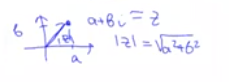
\includegraphics[width=180px]{pic00}
		\end{mylist}
	\begin{defin}
		$\forall x \in V \; \; \; $ \\
		\textbf{Длина вектора } $||x|| =\sqrt{(x, x)}$\\
		\textbf{Нормировать вектор} $\frac{x}{||x||} = x_0$ орт вектора, $||x_0|| = 1\\
		\forall x, y \neq \0 \; \; x, y \in V\\
		\phi$ -- угол между $x$ и $y: \cos\phi = \frac{(x, y)}{\|x\|\|y\|}$ (КБШ: $\frac{|(x, y)|}{\|x\|\|y\|} \leq 1$)
	\end{defin}
	\begin{examples}\ \\
		\begin{mylist}
			\item 
			$V_3$ геом. вект. $\underset{\text{скал}}{(x, y)} = |\vec x|\cdot |\vec y| \cdot \cos \phi$
			\item \belowbaseline[-11pt]{
			$\begin{matrix}
				\R^n (\mathbb C^n)\\
				x = \begin{pmatrix}
					x_1\\\vdots\\x_n
				\end{pmatrix} \in \R^n (\mathbb C^n)
			\end{matrix}$}$ \; \; \; (x, y) \ \underset{\text{(Евкл. } \sum x_i y_i \text{)}}{\sum\limits_{i=1}^n x_i \vec y_i}$ выполнены 1-4\\
			$(x, x) = \sum\limits_{i=1}^n x_i \vec x_i \ \sum\limits_i^n |x_i|^2
			 \begin{matrix}\geq 0\\
				=0 \Leftrightarrow \forall i\;  x_i = 0 \Leftrightarrow x = \0
			\end{matrix}\n
			||x|| = \sqrt{\sum|x_i|^2}$ евкл. норма\\
			КБШ: $|\sum\limits_i^n \vec{x_i y_i}| \leq (\sum\limits_i^n |x_i|^2)^{\frac{1}{2}} (\sum\limits_i^n|y_i|^2)^\frac{1}{2} \; \; \\
				\text{Нер-во треугольника:}\\
				(\sum\limits_i^n |x_i+y_i|^2)^\frac{1}{2} \leq (\sum\limits_i^n |x_i|^2)\frac{1}{2}
				+ (\sum\limits_i^n |y_i|^2)^\frac{1}{2}$
			\item 
			$f: [a, b] \rightarrow \mathbb C (\R) \; \; \; \; \; u, v \in \underset{\text{интегр.}}{R[a, b]} \; \; \int_{a}^{b} u(x) dx \; \int_{a}^{b} v(x) dx \n
			f = u + i v\n
			\int_{a}^{b} f dx = \int_{a}^{b} u dx + i \int_{a}^{b} v dx\n
			(\cdot, \cdot): V\times V \rightarrow \mathbb C \; \; \; \forall f, g \; \; (f, g) = \int_{a}^{b} f(x) \vec g(x) dx$\n
			Все аксиомы очевидно выполнены, есть проблемы с 4ой аксиомой.\n
			$(f, f) = \int_a^b |f|^2 dx \geq 0\n
			= 0 ? \Leftrightarrow f \equiv 0 $ почти везде на $[a, b]$\\
			Возникает \underline{евклидова норма}.\n
			$\|f\| = \sqrt{\int_a^b |f|^2 dx} \; \; \; L^2([a, b])$ -- пространство\n
			КБШ: $|\int_a^b f\vec g dx| \leq (\int_a^b |f|^2 dx)^\frac{1}{2} (\int_a^b |g|^2 dx)^\frac{1}{2}$ (Неравенство Буняковского)\n
			Неравенство треугольника: $(\int_a^b |f+g|^2 dx)^\frac{1}{2} \leq (\int_a^b |f|^2 dx)^\frac{1}{2} + (\int_a^b |g|^2 dx)^\frac{1}{2}$ \\
			(Неравенство Минковского)
		\end{mylist}
	\end{examples}
	\subsection{Процесс ортогонализации Грама-Шмидта. Ортонормированный базис (о.н.б.) 
		Ортогональные системы векторов.}
	$(V, (\cdot, \cdot))$ евклидово (унит.) пространство
	\begin{defin}
		$\forall x, y \in V \; \; $ ортогональные, если $(x, y) = 0$ \\(Очевидно, $\cos\phi = 0 \Rightarrow \phi = \pi/2 \leadsto $\underline{перпендикулярны})
	\end{defin}
	$\0$ ортогонален $\forall x \in V, \0$ ортогонален $V$\n
	$y \in V: \forall x \in V \; \; (y, x) = 0 \; \; $т.к. $\underset{x:=y}{(y, y) = 0} \Rightarrow y = \0$
	\begin{defin}
		$v_1 \ldots v_m$ \underline{попарно-ортогональны}, если $\forall i \neq j: (v_i, v_j) = 0$\n
		Система $v_1 \ldots v_m$ \underline{Ортонормированна}, если $\forall (i, j) \boxed{(v_i, v_j) = \delta_{ij}} = \left\{\begin{array}{c}
			1, i=j\\
			0, i\neq j
		\end{array}\right.$
	\end{defin}
	$\delta_{ij}$ -- символ Кронекера
	\begin{stat}
		$\underset{\text{ненулевые}}{v_1 \ldots v_m}$ \underline{попарно-ортог.}$\Rightarrow$ линейно незав.
	\end{stat}
	\begin{proof}
		$\sum\limits_{i=1}^n \alpha_i v_i = \0 \; \; \alpha_i \in K \; \; 0 = (\0, v_i) = (\sum\limits_{i=1}^m \alpha_i v_i, v_j) = \sum\limits_{i}^m \alpha_i (\overset{\neq 0 \ i=j}{v_i, v_j}) = \alpha_j (v_j, v_j) \neq 0 \n
		\Rightarrow \forall j \ \alpha_j = 0 \Rightarrow$ Линейно независ.
	\end{proof}
	\underline{Существует ли такая система?}\\
	$\exists ?$ о.н.с. в $V$ ?
	\begin{theorem}[Процесс ортогон. Грама-Шмидта]\ \\
		$\forall$ система векторов $a_1 \ldots a_m$ может быть заменена\\
		попарно-ортог. системой векторов $b_1 \ldots b_k$, с сохранением лин. оболочки\n
		$span(a_1 \ldots a_m) = span(b_1 \ldots b_k) \; \; k \leq m$
	\end{theorem}
	\begin{proof}\
		\begin{mylist}
			\item $a_1 \ldots a_m$ лин. незав.\\
			М.М.И.
			\begin{mylist}
				\item База индукции $m=1 \; \; a_1 = b_1$
				\item $\pu$ верно для $k-1$ вектора --- инд. предположение
				\item Инд. переход. Докажем для $k$ векторов.\n
				\begin{minipage}{150px}
					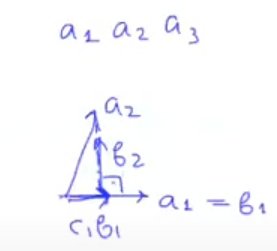
\includegraphics[width=150px]{pic01}
				\end{minipage}
				\begin{minipage}{300px}
					$b_2 = a_2 - c_1 b_1\\
					b_2 \perp b_1\\
					0 = (b_2, b_1) = (a_2, b_1) - c_1(b_1, b_1) \Rightarrow c_1 = \frac{(a_1, b_1)}{(b_1, b_1)}$
				\end{minipage}\\
				\begin{minipage}{150px}
					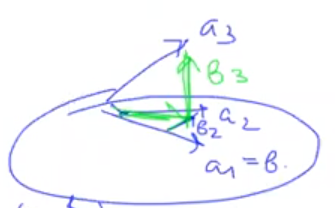
\includegraphics[width=150px]{pic02}
				\end{minipage}
				\begin{minipage}{300px}
					$b_3 = a_3 - \tilde{c_1} b_1 - \tilde{c_2} b_2\\
					(b_3, b_1) = 0 \; \; (b_3, b_2) = 0\n
					0 = (a_3, b_1) - \tilde{c_1}(b_1, b_1) \Rightarrow \tilde{c_1} = \frac{(a_3, b_1)}{(b_1, b_1)}\n
					0 = (a_3, b_2) - \tilde{c_2}(b_2, b_2) \Rightarrow \tilde{c_2} = \frac{(a_3, b_2)}{(b_2, b_2)}$
				\end{minipage}\n
				Теперь для $k$-мерного случая.\\
				$a_1 \ldots a_{k-1} \leadsto b_1 \ldots b_{k-1}$ попарно ортог.\\
				$\boxed{b_k = a_k - \sum\limits_{i=1}^{k-1} c_i b_i} \; \; \; \begin{matrix}
					c_i = ?\\
					(b_k, b_i) = 0 \; i = 1\ldots k-1
				\end{matrix}\n
				(b_k, b_j) = (a_k, b_j) - \sum\limits_{i=1}^{k-1} c_i (b_i, b_j) = (a_k, b_j) - c_j (b_j, b_j) \n
				\Rightarrow \boxed{c_j = \frac{(a_k, b_j)}{(b_j, b_j)}} \; \; j = 1 \ldots k-1\n
				\Rightarrow span(a_1 \ldots a_k) = span(\underset{\text{попарно-ортог.}}{b_1 \ldots b_k})$
			\end{mylist}
			\item 
			$a_1 \ldots a_m$ линейно зав. $\leadsto $ Г-Ш на каком-то этапе $b_j = \0$\n
			\slide{110px} $\leadsto$ проредить $a_1 \ldots a_m \leadsto \underset{\text{лин. независ.}}{a_{i_1}\ldots a_{i_k}} \leadsto$ Г-Ш.
		\end{mylist}
	\end{proof}
	\begin{corollary}
		В $\forall$ евкл. (унит.) пространстве $\exists$ О.Н.Б.(орто-нормир. базис)
	\end{corollary}
	\begin{proof}
		Упр.
	\end{proof}
	\begin{corollary}
		$\forall$ лин. независ. систему векторов евкл. (унит.) про-ва\\
		можно дополнить до о.н.б.
	\end{corollary}
	\begin{proof}
		Упр.
	\end{proof}
\end{document}